% Généré par analysis/analyse.py -- ne pas modifier à la main.
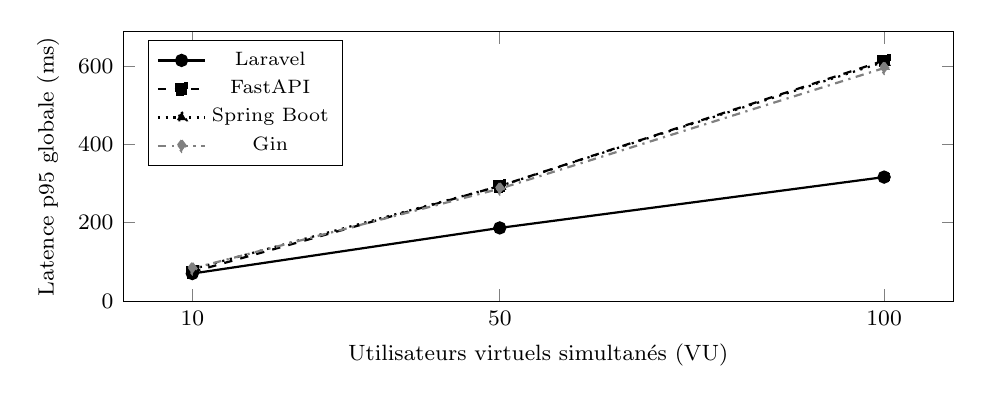
\begin{tikzpicture}
\begin{axis}[
  width=\columnwidth, height=5cm,
  xlabel={Utilisateurs virtuels simultanés (VU)},
  ylabel={Latence p95 globale (ms)},
  xtick={10,50,100},
  tick label style={font=\footnotesize},
  label style={font=\footnotesize},
  legend style={font=\scriptsize, at={(0.03,0.97)}, anchor=north west},
  ymin=0]
\addplot[black, thick, mark=*, error bars/.cd, y dir=both, y explicit]
  coordinates {(10,70.30) +- (0,0.30) (50,186.77) +- (0,2.26) (100,316.52) +- (0,9.65)};
\addplot[black, thick, dashed, mark=square*, error bars/.cd, y dir=both, y explicit]
  coordinates {(10,74.34) +- (0,0.51) (50,293.79) +- (0,6.64) (100,613.95) +- (0,10.71)};
\addplot[black, thick, dotted, mark=triangle*, error bars/.cd, y dir=both, y explicit]
  coordinates {(10,81.37) +- (0,0.22) (50,293.65) +- (0,0.95) (100,610.58) +- (0,9.72)};
\addplot[gray, thick, dashdotted, mark=diamond*, error bars/.cd, y dir=both, y explicit]
  coordinates {(10,83.21) +- (0,0.09) (50,286.87) +- (0,1.08) (100,594.91) +- (0,3.01)};
\legend{Laravel, FastAPI, Spring Boot, Gin}
\end{axis}
\end{tikzpicture}
